

\begin{frame}{\ft{AXFI Host Libraries and Application Integration}}
%\section{Research Slide 5}
\section{Host\\Libraries}
\doubleFrame{\normalsize{Complementary to AXFI Object Libraries, 
AXFI Host Libraries bridge Object Libraries with 
the applications where they are embedded.  The Host Library 
therefore shares computational resources with both 
the Co-Serialization Interface and the host GUI code.}}

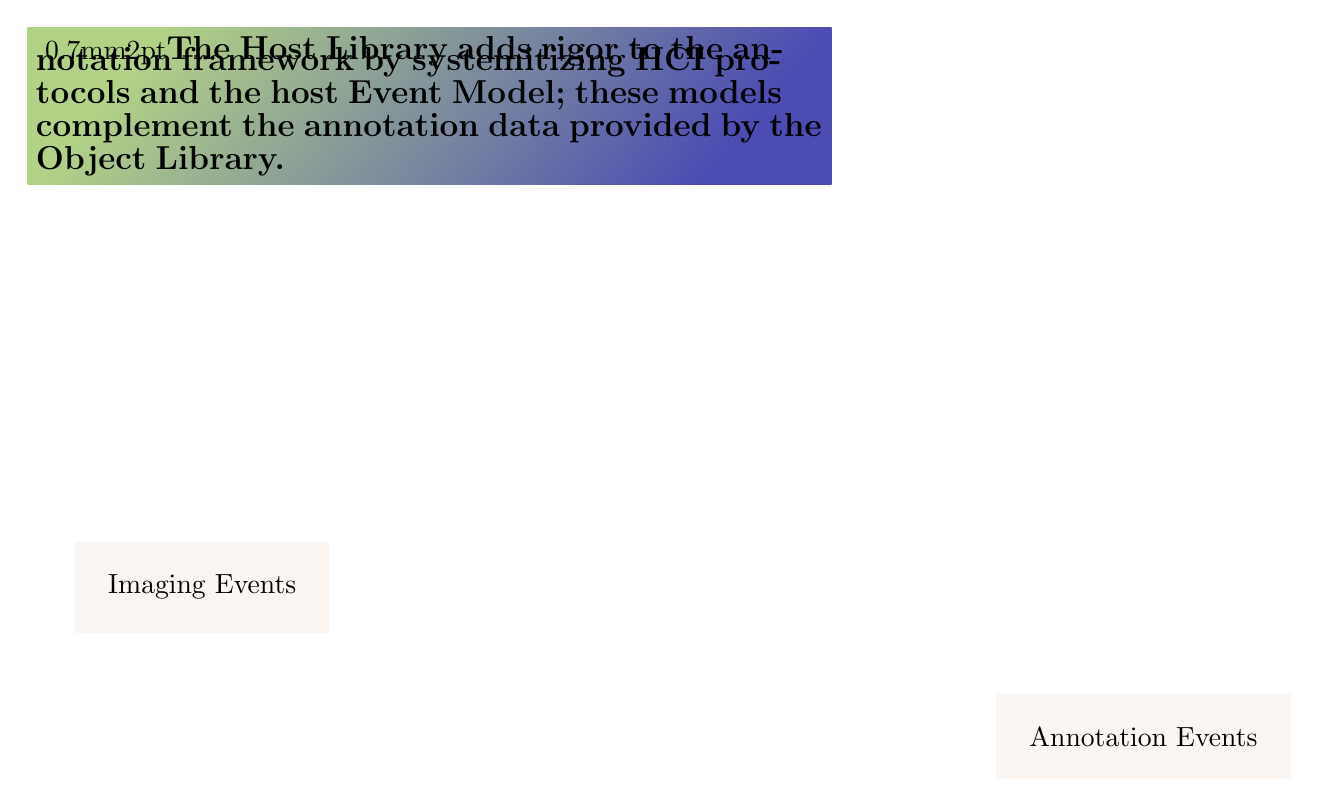
\begin{tikzpicture}
\nodeincludegraphicsTRRS{0.92}{0cm}{0cm}{0cm}{2cm}{pics/rad.png}

 \node [anchor=west,bottom color=yellow!30!blue,top color=pink!70!green, 
inner sep=3, shading angle=50, text width=10cm]
  (longnote) at (1.7,13.3) {\vspace{-8pt} %  %{\color{rb!85!red}{
  {\cframedboxx{0.7mm}{2pt}{\large\textbf{The Host Library 
adds rigor to the annotation framework by systemitizing 
HCI protocols and the host Event Model; these models 
complement the \makebox{annotation} data provided by the Object Library.}}}};

\rectann{darkRed}{0.7}{1mm}{grammarArrowColor}{0.5}{19,6}{3}{9.35}{0.9}

\node [anchor=west,fill=brown!8!white,inner sep=12, 
opacity=0.88, text opacity=1] (note) at (14,5.29) {\hc{Annotation Events}};

\ann{BlueGreen!90!red}{1}{.6mm}{blue!50!orange}{0.5}{1.21,8.2}{1.2}{2.6}{1.3}

\node [anchor=west,fill=brown!8!white,inner sep=12, 
opacity=0.88, text opacity=1] (inote) at (2.3, 7.19) {\hc{Imaging Events}};


\end{tikzpicture}


\end{frame}

